\iffalse
This file is protected by Copyright. Please refer to the COPYRIGHT file
distributed with this source distribution.

This file is part of OpenCPI <http://www.opencpi.org>

OpenCPI is free software: you can redistribute it and/or modify it under the
terms of the GNU Lesser General Public License as published by the Free Software
Foundation, either version 3 of the License, or (at your option) any later
version.

OpenCPI is distributed in the hope that it will be useful, but WITHOUT ANY
WARRANTY; without even the implied warranty of MERCHANTABILITY or FITNESS FOR A
PARTICULAR PURPOSE. See the GNU Lesser General Public License for more details.

You should have received a copy of the GNU Lesser General Public License along
with this program. If not, see <http://www.gnu.org/licenses/>.
\fi

% AV-5479: Assume this is in projects/assets_ts of source checkout
\def\importpath{../../../../assets/components/dsp_comps/complex_mixer.test/doc/}
\makeatletter
\def\input@path{{\importpath/snippets/}}
\makeatother
\documentclass{article}
\iffalse
This file is protected by Copyright. Please refer to the COPYRIGHT file
distributed with this source distribution.

This file is part of OpenCPI <http://www.opencpi.org>

OpenCPI is free software: you can redistribute it and/or modify it under the
terms of the GNU Lesser General Public License as published by the Free Software
Foundation, either version 3 of the License, or (at your option) any later
version.

OpenCPI is distributed in the hope that it will be useful, but WITHOUT ANY
WARRANTY; without even the implied warranty of MERCHANTABILITY or FITNESS FOR A
PARTICULAR PURPOSE. See the GNU Lesser General Public License for more details.

You should have received a copy of the GNU Lesser General Public License along
with this program. If not, see <http://www.gnu.org/licenses/>.
\fi

\author{} % Force author to be blank
%----------------------------------------------------------------------------------------
% Paper size, orientation and margins
%----------------------------------------------------------------------------------------
\usepackage{geometry}
\geometry{
	letterpaper,			% paper type
	portrait,				% text direction
	left=.75in,				% left margin
	top=.75in,				% top margin
	right=.75in,			% right margin
	bottom=.75in			% bottom margin
 }
%----------------------------------------------------------------------------------------
% Header/Footer
%----------------------------------------------------------------------------------------
\usepackage{fancyhdr} \pagestyle{fancy} % required for fancy headers
\renewcommand{\headrulewidth}{0.5pt}
\renewcommand{\footrulewidth}{0.5pt}
%----------------------------------------------------------------------------------------
% Appendix packages
%----------------------------------------------------------------------------------------
\usepackage[toc,page]{appendix}
%----------------------------------------------------------------------------------------
% Defined Commands & Renamed Commands
%----------------------------------------------------------------------------------------
\renewcommand{\contentsname}{Table of Contents}
\renewcommand{\listfigurename}{List of Figures}
\renewcommand{\listtablename}{List of Tables}
\newcommand{\todo}[1]{\textcolor{red}{TODO: #1}\PackageWarning{TODO:}{#1}} % To do notes
\newcommand{\code}[1]{\texttt{#1}} % For inline code snippet or command line
%----------------------------------------------------------------------------------------
% Various pacakges
%----------------------------------------------------------------------------------------
\usepackage{hyperref} % for linking urls and lists
\usepackage{graphicx} % for including pictures by file
\usepackage{listings} % for coding language styles
\usepackage{rotating} % for sideways table
\usepackage{pifont}   % for sideways table
\usepackage{pdflscape} % for landscape view
%----------------------------------------------------------------------------------------
% Table packages
%----------------------------------------------------------------------------------------
\usepackage{longtable} % for long possibly multi-page tables
\usepackage{tabularx} % c=center,l=left,r=right,X=fill
\usepackage{float}
\floatstyle{plaintop}
\usepackage[tableposition=top]{caption}
\newcolumntype{P}[1]{>{\centering\arraybackslash}p{#1}}
\newcolumntype{M}[1]{>{\centering\arraybackslash}m{#1}}
%----------------------------------------------------------------------------------------
% Block Diagram / FSM Drawings
%----------------------------------------------------------------------------------------
\usepackage{tikz}
\usetikzlibrary{shapes,arrows,fit,positioning}
\usetikzlibrary{automata} % used for the fsm
\usepackage{amsmath}
%----------------------------------------------------------------------------------------
% Colors Used
%----------------------------------------------------------------------------------------
\usepackage{colortbl}
\definecolor{blue}{rgb}{.7,.8,.9}
\definecolor{ceruleanblue}{rgb}{0.16, 0.32, 0.75}
\definecolor{drkgreen}{rgb}{0,0.6,0}
\definecolor{deepmagenta}{rgb}{0.8, 0.0, 0.8}
\definecolor{cyan}{rgb}{0.0,0.6,0.6}
\definecolor{maroon}{rgb}{0.5,0,0}

%----------------------------------------------------------------------------------------
% Update the docTitle and docVersion per document
%----------------------------------------------------------------------------------------
\def\docTitle{Component Data Sheet}
\def\docVersion{1.5}
%----------------------------------------------------------------------------------------
\date{Version \docVersion} % Force date to be blank and override date with version
\title{\docTitle}
\lhead{\small{\docTitle}}

\def\comp{complex\_mixer\_ts}
\edef\ecomp{complex_mixer_ts}
\def\Comp{Complex Mixer (TimeStamped)}
\graphicspath{ {\importpath/figures/} }

\begin{document}

\section*{Summary - \Comp}
\begin{tabular}{|c|M{13.5cm}|}
	\hline
	\rowcolor{blue}
	                  & \\
	\hline
	Name              & \comp \\
	\hline
	Worker Type       & Application \\
	\hline
	Version           & v\docVersion \\
	\hline
	Release Date      & 4/2019 \\
	\hline
	Component Library & ocpi.assets\_ts.components \\
	\hline
	Workers           & \comp.hdl \\
	\hline
	Tested Platforms  & xsim, isim, modelsim, Matchstiq-Z1(PL) \\
	\hline
\end{tabular}
\section*{Functionality}
\begin{flushleft}
	The Complex Mixer consists of a Numerically Controlled Oscillator (NCO) and a complex multiplier. Complex IQ data is received on the input port and is multiplied with the output of the NCO and put on the output port.
\end{flushleft}

\section*{Worker Implementation Details}
\subsection*{\comp.hdl}
\begin{flushleft}
	Figure \ref{fig:complex_mixer} diagrams the complex mixer.\medskip

	\begin{figure}[h]
		\centering\captionsetup{type=figure}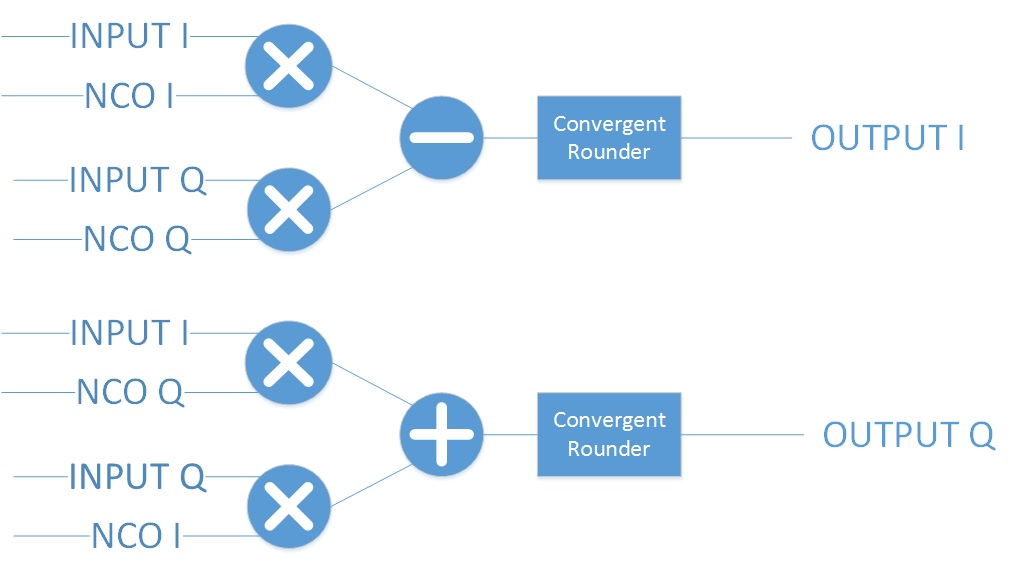
\includegraphics[scale=0.4]{complex_mixer_block_diagram}
		\captionof{figure}{Complex Mixer Functional Diagram}
		\label{fig:complex_mixer}
	\end{figure}
	Build time parameters can be used to control the width of the NCO data output, the width of the input data, and the number of stages in the Coordinate Rotation Digital Computer (CORDIC) used to implement the NCO. Additionally, there is a parameter to control insertion of a peak detection circuit.\medskip

	An \verb+enable+ input is available to either enable (true) or bypass (false) the circuit. In bypass mode, pipe-lining registers are not used. FPGA multipliers are used to process input data at the full clock rate. This worker will produce valid output two clock cycles after each valid input.
\end{flushleft}

\section*{Theory}
\begin{flushleft}
	The Complex Mixer worker inputs complex signed samples and performs a complex multiply with a digital sine wave produced by an numerically controlled oscillator (NCO). The resulting output data is a frequency shifted version of the input data.\medskip

	The magnitude of the frequency shift is determined by the output frequency of the NCO, which can be calculated with the following equation:

	\begin{equation} \label{eq:nco_output_freq}
		nco\_output\_freq = sample\_freq*\frac{phs\_inc}{2^{phs\_acc\_width}}
	\end{equation}

	In this component, \verb+phs_inc+ is runtime configurable and has a data type of 16 bit signed short. \verb+phs_acc_width+ is fixed at 16. The input clock frequency is the sample rate of the samples. The amplitude of the NCO's sine wave is also runtime configurable via the \verb+mag+ property. Note that the \verb+mag+ property value should only ever be set to a value within the following range in order for the worker to operate properly.

	\begin{equation} \label{eq:mag_limits_freq}
		-2^{(NCO\_DATA\_WIDTH\_p-1)} <= mag <= 2^{(NCO\_DATA\_WIDTH\_p-1)}-1
	\end{equation}

	A positive and negative \verb+phs_inc+ will mix up and down, respectively. The following equation can be used as an aid for setting the \verb+phs_inc+ to have the desired mixing affect.\medskip

	\begin{equation} \label{eq:positive_phs_inc_mixes_up}
		x_{out}[n] = x_{in}[n] * \dfrac{mag}{2^{NCO\_DATA\_WIDTH\_p-1}} * e^{\big(j2\pi\big(sample\_freq * \dfrac{phs\_inc \; * \; n}{2^{phs\_acc\_width}}\big) + phs\_init\big)} \;\; \forall \;\; n, \; n \ge 0
	\end{equation}

\end{flushleft}


\section*{Block Diagrams}
\subsection*{Top level}
	\begin{center}
		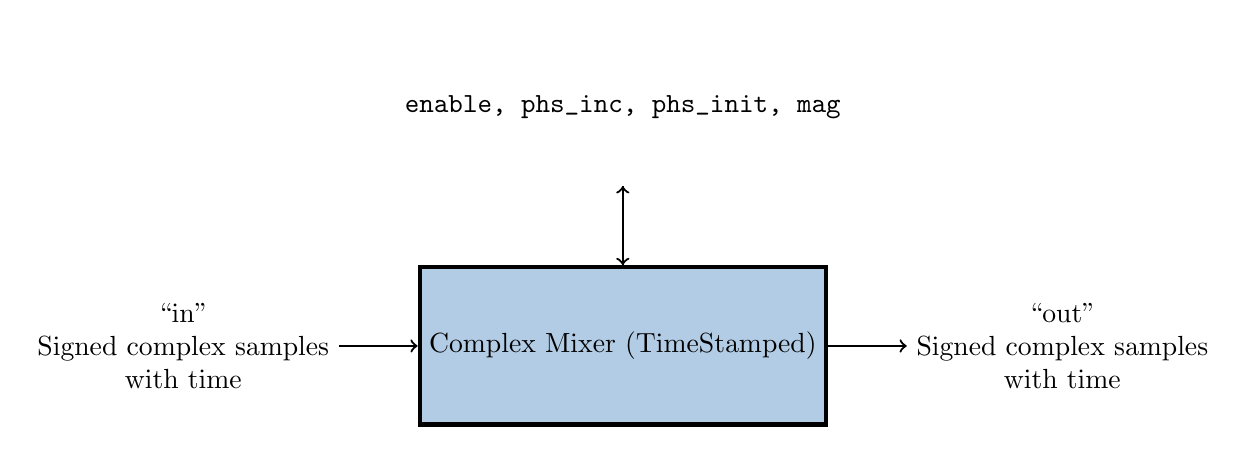
\begin{tikzpicture}[% List of styles applied to all, to override specify on a case-by-case
				every node/.style={
					align=center,  		% use this so that the "\\" for line break works
					minimum size=2cm	% creates space above and below text in rectangle
				},
				every edge/.style={draw,thick}
			]
			\node[rectangle,ultra thick,draw=black,fill=blue](R2){\Comp};
			\node[rectangle,draw=white,fill=white](R3)[left= of R2]{``in'' \\ Signed complex samples \\ with time};
			\node[rectangle,draw=white,fill=white](R4)[right= of R2]{``out'' \\ Signed complex samples \\ with time};
			\node[rectangle,draw=white,fill=white](R5)[above= of R2]{\verb+enable, phs_inc, phs_init, mag+};
			\path[->]
			(R3)edge []	node [] {} (R2)
			(R2)edge []	node [] {} (R4)
			(R2)edge []	node [] {} (R5)
			(R5)edge []	node [] {} (R2)
			;
		\end{tikzpicture}
	\end{center}
	\captionof{figure}{Complex Mixer Top Level Block Diagram}
	\label{fig:block_diagram}

\newpage
\section*{Source Dependencies}
\subsection*{\comp.hdl}
\begin{itemize}
	\item projects/assets\_ts/components/complex\_mixer.hdl/complex\_mixer.vhd
        	\item projects/assets/hdl/primitives/dsp\_prims/dsp\_prims\_pkg.vhd
	      \subitem projects/assets/hdl/primitives/dsp\_prims/nco/src/nco.vhd
	      \subitem projects/assets/hdl/primitives/dsp\_prims/cordic/src/cordic\_pr.vhd
	      \subitem projects/assets/hdl/primitives/dsp\_prims/cordic/src/cordic.vhd
	      \subitem projects/assets/hdl/primitives/dsp\_prims/cordic/src/cordic\_stage.vhd
	\item projects/assets/hdl/primitives/util\_prims/util\_prims\_pkg.vhd
	      \subitem projects/assets/hdl/primitives/util\_prims/mult/src/complex\_mult.vhd
	      \subitem projects/assets/hdl/primitives/util\_prims/pd/src/peakDetect.vhd
	\item projects/assets/hdl/primitives/misc\_prims/misc\_prims\_pkg.vhd
	      \subitem projects/assets/hdl/primitives/misc\_prims/round\_conv/src/round\_conv.vhd

\end{itemize}

\begin{landscape}
	\section*{Component Spec Properties}
	\begin{scriptsize}
		\begin{tabular}{|p{3cm}|p{1.5cm}|c|c|c|p{1.5cm}|p{1cm}|p{7cm}|}
			\hline
			\rowcolor{blue}
			Name               & Type   & SequenceLength & ArrayDimensions & Accessibility	& Valid Range	& Default 	& Usage\\
			\hline
			\verb+enable+      & bool   & -              & -               & Writable			& -				& true    	& Enable(true) or bypass(false) mixer\\
			\hline
			\verb+phs_inc+     & short  & -              & -               & Writable			& -				& -4096		& Phase increment of NCO\\
			\hline
		\end{tabular}
	\end{scriptsize}

	\section*{Worker Properties}
	\subsection*{\comp.hdl}
	\begin{scriptsize}
		\begin{tabular}{|p{1.5cm}|p{2.5cm}|p{1cm}|c|c|c|p{2cm}|p{1cm}|p{5cm}|}
			\hline
			\rowcolor{blue}
			Type     & Name                      	& Type  	& SequenceLength & ArrayDimensions & Accessibility	& Valid Range 	& Default & Usage\\
			\hline
			Property & \verb+NCO_DATA_WIDTH_p+		& uchar 	& -              & -               & Parameter		& 12/16       	& 12      & Output data width of NCO\\
			\hline
			Property & \verb+INPUT_DATA_WIDTH_p+	& uchar 	& -              & -               & Parameter		& 12/16       	& 12      & Input port data width\\
			\hline
			Property & \verb+CORDIC_STAGES_p+    	& uchar 	& -              & -               & Parameter		& 16          	& 16      & Number of CORDIC stages implemented in NCO\\
			\hline
			Property & \verb+PEAK_MONITOR_p+     	& bool  	& -              & -               & Parameter		& -				& true    & Include peak monitor circuit\\
			\hline
			Property & \verb+LATENCY_p+     	  	& ushort	& -              & -               & Parameter		& 2				& 2		  & Number of clock cycles between a valid input and a valid output\\
			\hline
			Property & \verb+peak+            		& short 	& -              & -               & Volatile		& -				& -       & Output of peak detector\\
			\hline
			Property & \verb+phs_init+    			& ushort 	& -              & -               & Writable 		& -           	& 0       & Initial phase of NCO\\
			\hline
			Property & \verb+mag+         			& ushort 	& -              & -               & Writable 		& -           	& 1024    & Magnitude of NCO output\\
			\hline
		\end{tabular}
	\end{scriptsize}

	\section*{Component Ports}
	\begin{scriptsize}
		\begin{tabular}{|M{2cm}|M{1.5cm}|M{4cm}|c|c|M{9cm}|}
			\hline
			\rowcolor{blue}
			Name & Producer & Protocol         				& Optional	& Advanced & Usage\\
			\hline
			in   & -		& Complex\_Short\_With\_Metadata	& -			& -        & Signed complex samples\\
			\hline
			out  & -		& Complex\_Short\_With\_Metadata	& -			& -        & Signed complex samples\\
			\hline
		\end{tabular}
	\end{scriptsize}

	\section*{Worker Interfaces}
	\subsection*{\comp.hdl}
	\begin{scriptsize}
		\begin{tabular}{|M{2cm}|M{1.5cm}|c|c|M{12cm}|}
			\hline
			\rowcolor{blue}
			Type            & Name & DataWidth & Advanced  & Usage\\
			\hline
			StreamInterface & in   & 32        & -			& Signed Complex Samples\\
			\hline
			\rowcolor{blue}
			Type            & Name & DataWidth & Advanced	& Usage\\
			\hline
			StreamInterface & out  & 32        & 			& Signed Complex Samples\\
			\hline
		\end{tabular}
	\end{scriptsize}
\end{landscape}

\section*{Control Timing and Signals}
\begin{flushleft}
	The Complex Mixer HDL worker uses the clock from the Control Plane and standard Control Plane signals.\medskip

	There is a startup delay for this worker. Once the input is ready and valid and the output is ready, there is a delay of \verb+CORDIC_STAGES_p++1 before the first sample is taken. After this initial delay, valid output data is given 2 clock cycles after input data is taken.

	\begin{tabular}{|M{4.5cm}|M{1cm}|M{1cm}|M{1.5cm}|M{2cm}|M{1cm}|M{1cm}|M{2.5cm}|}
		\hline
		\rowcolor{blue}
		Latency         \\
		\hline
		2 clock cycles  \\
		\hline
	\end{tabular}
\end{flushleft}

\begin{landscape}
\section*{Worker Configuration Parameters}
\subsubsection*{\comp.hdl}
f\input{../../\ecomp.hdl/configurations.inc}
\section*{Performance and Resource Utilization}
\input{../../\ecomp.hdl/utilization.inc}
\end{landscape}
\section*{Test and Verification}
Test cases are derived from the number of properties, and their respective values, as listed in the \comp-test.xml.
\begin{itemize}
	\item[1)] Bypass: The input data is forwarded to the output port. For verification of this case, the output file is byte-wise compared to the input file.
	\item[2)] Normal mode:
	Input data is generated by first creating a *.dat input file containing all of the operations of the Complex\_Short\_With\_Metadata protocol in the following sequence:
\begin{enumerate}
	\item Interval
	\item Sync (this opcode is expected after an Interval operation)
	\item Time
	\item Samples (tone with configurable length and magnitude)
	\item Flush	
	\item Samples (tone with configurable length and magnitude)
	\item Sync
	\item Samples (tone with configurable length and magnitude)
\end{enumerate}
The samples messages consist of a tone with configurable length and magnitude.\medskip

The NCO is configured to tune the input samples operations to baseband. For verification, an FFT of the output data is performed and the max value of the FFT is checked to be at DC (0 Hz).\medskip

The worker will pass through all operations of the Complex\_Short\_With\_Metadata protocol. During sync operations, the NCO is reset.

\end{itemize}

\end{document}
